\chapter{Vorstellung der vorhanden Hardware}
\label{sec:Hardware}
Die Hardware besteht im wesentlichen aus den Komponenten in Abbildung \ref{fig:Übersicht}.
\todo{Nummern oder Farben in Bild!}
\begin{figure}[htb]
\centering
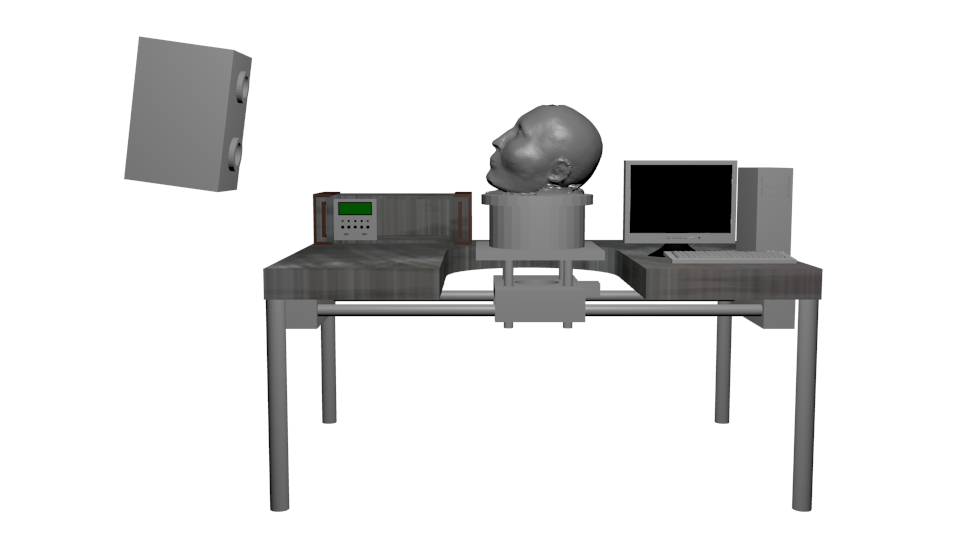
\includegraphics[width=\textwidth]{Blender/Schema_Arbeitsplatz.png}
\caption{Blick auf den Arbeitsaufbau}
\label{fig:Übersicht}
\end{figure}
\todo{ Komponenten auf Abbildung erwähnen!}

\section{Computer}
Zur Verfügung steht ein IBM kompatibler x86 Standard PC mit einer SCSI-Schnittstelle und zwei seriellen RS-232-Schnittstellen. 

\section{3D-Laserscanner VI-900}
\begin{figure}[htb]
\centering
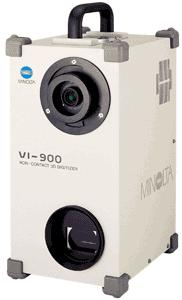
\includegraphics[width=100pt]{vi900-big.jpg}
\caption{VI-900 - 3D-Scanner}
\label{fig:VI900}
\end{figure}
Der 3D-Laserscanner \Fachbegriff{VI-900} der Firma Minolta besteht, wie auf Abbildung \ref{fig:VI900} zu sehen, aus einem \Fachbegriff{Lasertriangulator}(unten) und einer Kamera(oben). Das System lässt sich über eine \Fachbegriff{SCSI}-Schnittstelle ansprechen und konfigurieren. Zur mobilen Nutzung kann das Gerät auch auf der Rückseite bedient werden. Aufgenommene Daten können auf einer \Fachbegriff{CF-Karte} gespeichert werden. Im Projekt wurde jedoch lediglich die direkte Ansteuerung via SCSI genutzt.
\subsection{Lasertriangulator Prinzip}
Ein Lasertriangulator, wie in Abbildung \ref{fig:LaserTriangulator} zu sehen, besteht aus einem Laser, einem Linsensystem und im einfachsten Fall aus einer Pixeldetektorzeile. Der Laser strahlt auf ein Objekt und je nach Entfernung des Objektes wird das Streulicht unter einem anderen Winkel zurückgestrahlt. Das Streulicht wird durch die Linsen auf den Pixeldetektor abgebildet. Über die Position des Laserspots auf dem Pixeldetektor lässt sich auf die Entfernung des Objektes schließen.\\
Der VI-900 digitalisiert Objekte durch ein Laser-Lichtschnittverfahren. Das vom Objekt reflektierte Licht wird von einer CCD-Flächenkamera erfasst, nach Ermittlung der Distanzwerte (Z-Achse) mittels Laser-Triangulation werden die 3D-Daten erstellt. Der Laserstrahl wird mit Hilfe eines hochpräzisen galvanischen Spiegels über das Objekt projiziert, pro Scan werden 640 x 480 Einzelpunkte erfasst.\cite{Minolta:Einleitung}\\
Die Technischen Daten befinden sich im Anhang in Tabelle \ref{tab:TD_VI-910}
\begin{figure}[htb]
\centering
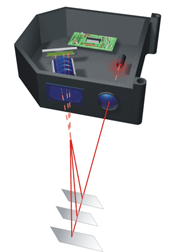
\includegraphics[width=100pt]{Laser-Triangulation.png}
\caption{Prinzip: Laser-Triangulation}
\label{fig:LaserTriangulator}
\end{figure}
\section{Ansteuerung für den Drehtisch}
Die Ansteuerung für den Drehtisch ist in einem 19''-Rack verbaut(siehe Abbildung \ref{fig:19Zoll_Rack}).
\begin{figure}[htb]
\centering
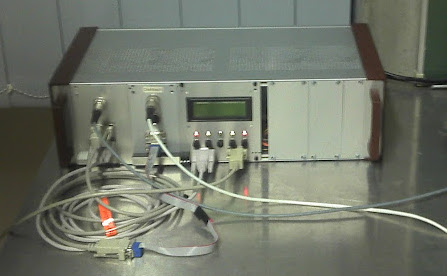
\includegraphics[width=100pt]{19Zoll_Rack}
\caption{Ansteuerung im 19''-Rack}
\label{fig:19Zoll_Rack}
\end{figure}
\subsection{Drehtisch}
\begin{figure}[htb]
\centering
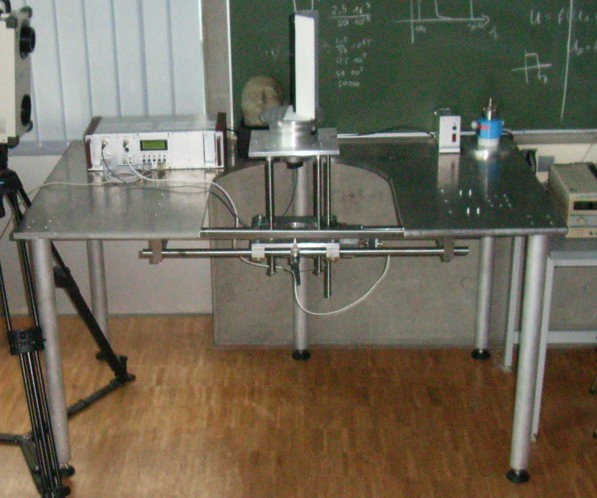
\includegraphics[width=100pt]{Drehtisch}
\caption{Drehtisch}
\label{fig:Drehtisch}
\end{figure}
Der Drehtisch(siehe Abbildung \ref{fig:Übersicht}) ist eine Eigenkonstruktion der Werkstatt des RheinAhrCampus. Er besteht aus einer massiven Edelstahl Arbeitsplatte, welche auf 4 Füßen ruht. Aus dieser ist ein Rechteck mit aufgesetztem Halbkreis ausgeschnitten. In diesem Ausschnitt befindet sich der Drehtisch. Er ist auf einem Schienensystem gelagert. Mit dem Schienensystem kann der Drehtisch in der Vertikalen positioniert werden. Mit einem Schrittmotor lässt sich der Drehtisch zusätzlich in der Höhe verstellen. Die Höhenverstellung wird mit einem \Fachbegriff{Schneckengetriebe} realisiert. Ein weiterer Schrittmotor ist für die Drehung des Tisches zuständig. Der Tisch ist über ein \Fachbegriff{Harmonic-Drive-Getriebe} mit dem Schrittmotor verbunden. Das Übersetzungsverhältnis beträgt 1:50.  
 
\subsection{Spannungsversorgung}
Die Schrittmotorkarten werden von einem PC-Netzteil gespeist. Die \Fachbegriff{Logikbausteine} werden mit 5V gespeist, zusätzlich werden die Schrittmotorkarten mit 12V für die Schrittmotoren gespeist. Die Kabel sind direkt an die \todo{Verbindungsleisten} gelötet.\\
Dies verhindert das einfache Ausbauen der Spannungsversorgung und die einfache Erweiterung um neue Einschubkarten.
%Um den Aufbau modular und erweiterbar zu machen, ersetzte ich die feste Lötverbindung durch eine Standard PC-Netzteil Verbindung(siehe Abbildung \ref{fig:Y-Kabel}). Dadurch kann das Netzteil nun einfach ausgebaut werden, bzw. das System leicht mit neuen Einschubkarten erweitert werden.\\
%Die \Fachbegriff{Logikbausteine} der Schrittmotorkarten und die Mikrocontroller-Platine werden mit 5V gespeist. Zusätzlich werden die Schrittmotorkarten mit 12V für die Schrittmotoren gespeist.
%\begin{figure}[htb]
%\centering
%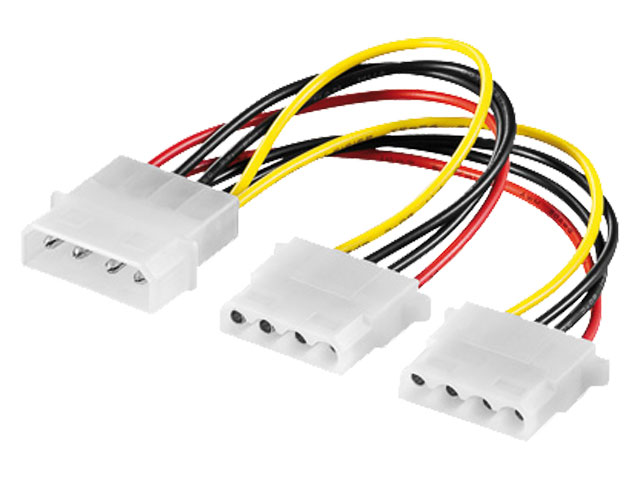
\includegraphics[width=100pt]{Y-Kabel.jpg}
%\caption{Stromverbinder - Y-Kabel}
%\label{fig:Y-Kabel}
%\end{figure}
%\todo{\url{http://www.kosatec.de/prod_images/kc/640x480/100539.jpg}}
\subsection{Schrittmotoren}
\todo{Motoren beschreiben! Technische Daten! Schritte, Spannungen. Verdrahtung.}

\subsection{Schrittmotorkarten}
Die Ansteuerung für die Schrittmotoren sind als 19''-Einschübe realisiert. Für jeden Schrittmotor wird ein Einschub benötigt.
Die Einschübe sind Produkte der Firma R+S. Mittels \Fachbegriff{RS-232 Schnittstelle} lassen sich die Karten konfigurieren und ansteuern. Die Konfiguration und Ansteuerung erfolgt über einen vorgegeben 
\Fachbegriff{ASCII}\footnote{Der American Standard Code for Information Interchange (ASCII, alternativ US-ASCII, oft [æski] ausgesprochen) ist eine 7-Bit-Zeichenkodierung\cite{wiki:ASCII}}
 Befehlssatz. Der Befehlssatz befindet sich im Kapitel \ref{sec:A_ASCII_Befehle}. Es können zwei oder mehr Karten als 
\Fachbegriff{Daisy-Chain}\footnote{Als Daisy Chain (englisch, wörtlich „Gänseblümchenkette“) bezeichnet man eine Anzahl von Hardware-Komponenten, welche in Serie miteinander verbunden sind (meist in sogenannten Bussystemen in der Automatisierungstechnik).\cite{wiki:Daisy} } 
in Reihe geschaltet werden.
\subsection{Motorverkabelung}
Die Schrittmotoren benötigen ein mindestens 4-adriges Kabel. Das Kabel für den Schrittmotor, der für die Rotation zuständig ist, war bereits gefertigt. Ein Kabel zwischen Schrittmotor und Schrittmotorkarte zur Höhenverstellung und für die Endschalter ist nicht vorhanden. 

%Hier wurden 3 weitere Adern für die beiden Endschalter benötigt.\\ Abbildung \ref{fig:Motorverkabelung} zeigt eine schematische Darstellung des Kabel. Tabelle \ref{tab:Motorverkabelung} gibt die Belegung der Kabel wieder.\todo{Belegung überprüfen!}
%\begin{figure}[htb]
%\centering
%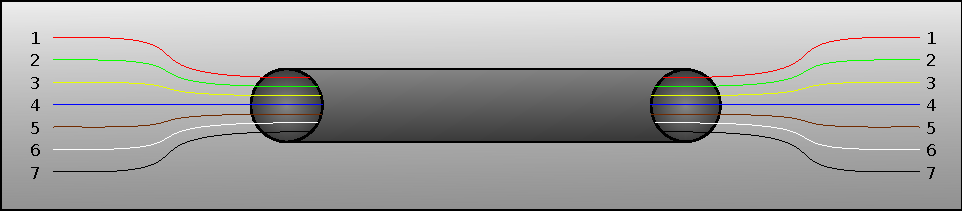
\includegraphics[width=\textwidth]{Kabel.pdf}
%\caption{Motor- und Endschalterverkabelung}
%\label{fig:Motorverkabelung}
%\end{figure}
%\begin{longtable}{|c|l|} 
%\caption{Motor- und Endschalterverkabelung} \\
%\hline
%\label{tab:Motorverkabelung}
%1 & Phase A \\ 
%\hline 
%2 & Phase B \\ 
%\hline 
%3 & Phase C \\ 
%\hline 
%4 & Phase D \\ 
%\hline 
%5 & Endschalter oben \\ 
%\hline 
%6 & Endschalter unten \\ 
%\hline 
%7 & Endschalter Masse \\ 
%\hline 
%\end{longtable} 

\subsection{Endschalter}
Die Schrittmotorkarten unterstützen das Abschalten der Motoren wenn ein sogenannter Endschalter ausgelöst wird. Dies sind im allgemeinen mechanische Schalter die ausgelöst werden wenn der Tisch sich dem Ende des Arbeitsbereiches nähert. Dies verhindert eine Beschädigung des Aufbaus.\\
Im Aufbau sind bereits induktive Endschalter der Firma \textit{Pepperl+Fuchs} verbaut. 
Am Drehtisch ist ein Metallstutzen von ungenügender Länge angebracht. Durch die ungenügende Länge des Metallstutzen würde der Endschalter nicht rechtzeitig ausgelöst werden und der Aufbau des Drehtisches würde beschädigt.

%Normalerweise unterstützt die Schrittmotorkarte nur mechanische Endschalter. Durch geschickte Verdrahtung ließen sich die induktiven Endschalter verwenden. Hierzu musste über einen Spannungsteiler die Spannung herabgesetzt werden. Dadurch konnten die Endschalter direkt an die Optokoppler der Schrittmotorkarte angeschlossen werden. 
%\begin{figure}[htb]
%\centering
%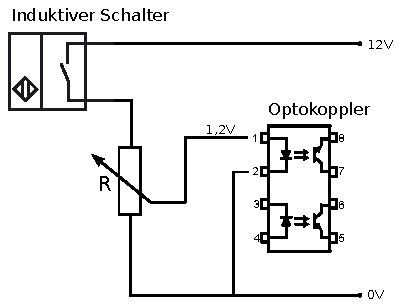
\includegraphics{Endschalter.pdf}
%\caption{Motor- und Endschalterverkabelung}
%\label{fig:Motorverkabelung}
%\end{figure}\\
% Zur Abhilfe lies ich einen längeren Metallstutzen von der Werkstatt anfertigen.\\
%Wenn der Tisch sich in der Endposition befindet, soll dies auch auf dem Mikrocontroller angezeigt werden. Die Signale der Endschalter liegen auf der Rückseite der Schrittmotorkarte \todo{Zeichnung der Anschlüsse referenzieren.} am Verbindungsstecker an. Ich lötete eine Brücke zwischen den Verbindungssteckern der Schrittmotorkarte und des Mikrocontrollers.\\
%Auf der Mikrocontrollerplatine sind diese Pins mit dem Mikrocontroller verbunden. Die beiden Pins werden im Mikrocontroller als \Fachbegriff{Interrupts} definiert. Die Interrupt-Service-Routine wird in Kapitel \ref{sec:Interrupts} beschrieben.

\section{Mikrocontroller}
Ein \Fachbegriff{Mikrocontroller} vereint, in einem IC, die wichtigsten Komponenten um komplexe technische Probleme leicht lösen zu können. Dazu gehören z.B. CPU, Flash-Speicher, Arbeitsspeicher, Register, Ports, ADC, DAC und mehr. Einen schematischen Überblick über die Komponenten eines Mikrocontrollers bietet das Blockdiagramm in Abbildung \ref{fig:uC_Blockdiagramm}. \\
%Um den Mikrocontroller nutzen zu können ist es notwendig den Mikrocontroller mit einem Programm zu beschreiben(\Fachbegriff{Flashen}). Dies lässt sich am einfachsten in einer Entwicklungsumgebung(siehe Kapitel \ref{sec:Entwicklungsumgebung}). Diese Programme können dann z.B. Signale an Pins des Mikrocontrollers auswerten und Signale über andere Pins wieder ausgeben und dadurch externe Geräte steuern. Eingehende Signale können binär ausgewertet,  oder mit einem ADC die Spannungshöhe bestimmt werden. Ausgehende Signale können auch binär oder mit einem DAC analog ausgegeben werden. Binäre Signale können zur Steuerung von LEDs oder Peripherie-Geräten genutzt werden. Auch LC-Displays und serielle Schnittstellen können so angesteuert werden. \todo{Umstellungsprobleme}
Für unterschiedliche Aufgaben sind unterschiedliche Mikrocontroller geeignet.\\
Es steht ein ATmega8515\cite{atmel:8515} im DIL-Gehäuse zur Verfügung. Dieser hat 8 Kbyte Flash, drei externe Interrupts, eine serielle Schnittstelle und kann mit bis zu 16 MHz betrieben werden. 
Dieser ist geeignet um sich in die Programmierung mit \Fachbegriff{C} einzufinden und eine serielle Schnittstelle anzusteuern. \\
Für dieses Projekt sind jedoch zwei serielle Schnittstellen nötig. Der ATmega 324A\cite{atmel:324A} würde diese Voraussetzungen erfüllen, ist jedoch nicht vorhanden. Er ist dem ATmega 8515 recht ähnlich, bietet jedoch die benötigten zwei seriellen Schnittstellen. Des Weiteren hat er 32 Kbyte Flash. 
%Diese wurden aufgrund des recht umfangreichen Programms und der diversen Bibliotheken notwendig.
\begin{figure}[htb]
\centering
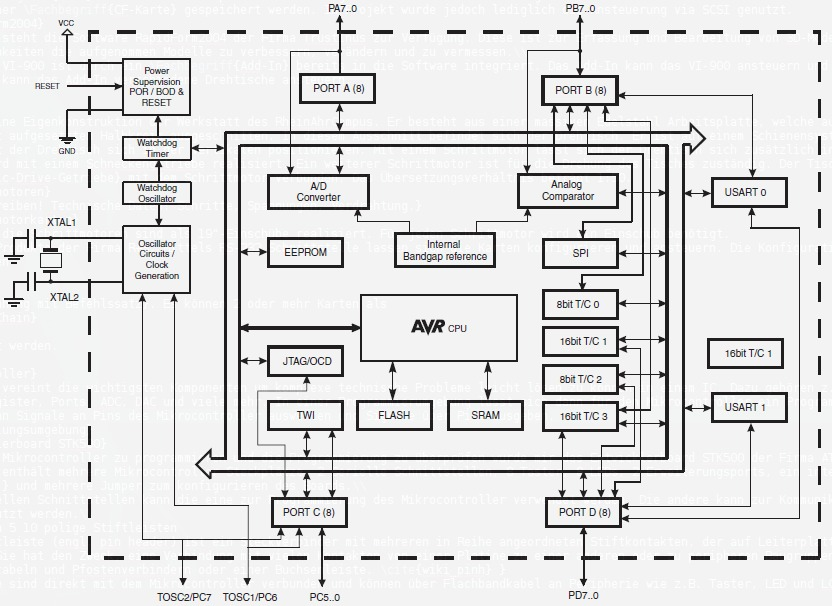
\includegraphics[width=\textwidth]{uC_Block}
\caption{Block Diagram: Mikrocontroller}
\label{fig:uC_Blockdiagramm}
\citep{atmel:ug_324A}
\end{figure}
\subsection{Entwicklerboard STK500}
Um den Mikrocontroller zu programmieren und die Programmierung zu überprüfen, soll das \Fachbegriff{Entwicklerboard STK500}(siehe Abbildung \ref{fig:STK500}) der Firma ATMEL verwendet werden. Das Board enthält mehrere Mikrocontroller-Steckplätze, 2 serielle Schnittstellen, 8 Taster, 8 LEDs, 2 Erweiterungsports, eine Programmierschnittstelle \Fachbegriff{ISP}\footnote{In System Programmer} und mehrere Jumper zum Konfigurieren des Boards.\\
Von den beiden seriellen Schnittstellen kann die eine zur Programmierung des Mikrocontrollers verwendet werden. Die andere kann zur Kommunikation mit dem Mikrocontroller genutzt werden.\\
Auf dem Board stehen fünf 10 polige Stiftleisten 
zur Verfügung. Diese sind direkt mit den Ports des Mikrocontroller verbunden und können über Flachbandkabel mit \todo{Peripherie} wie z.B. Taster, LED, LC-Displays oder seriellen Schnittstellen verbunden werden.
\begin{figure}[htb]
\centering
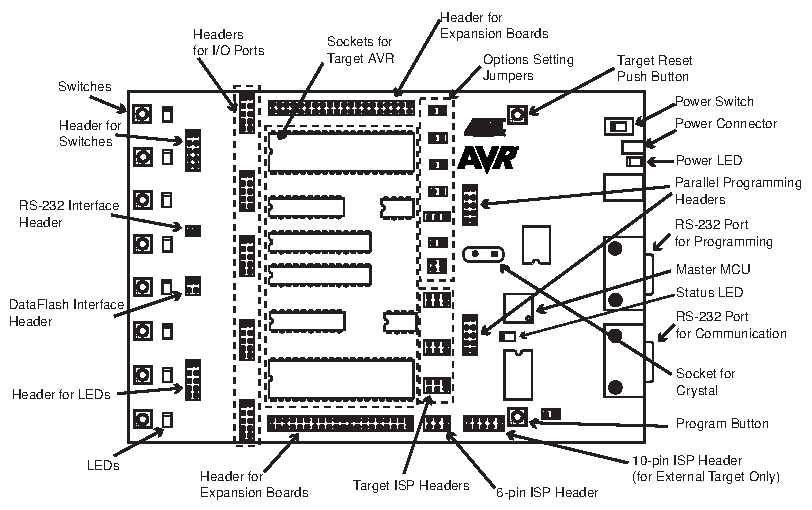
\includegraphics[width=\textwidth]{STK500_Schema.pdf}
\caption{Schema: STK500}
\label{fig:STK500}
\citep{atmel:ug_STK500}
\end{figure}

\subsection{AVRISP mkII}
Das AVRISP mkII ist ein USB-basiertes \Fachbegriff{In-System-Programmiersystem}. Dieses kann anstelle des RS-232 basierten Programmiersystem des STK500 verwendet werden.\\
Die Übertragungsgeschwindigkeit des AVRISP mkII ist wesentlich höher als die der Seriellen Schnittstelle. 
%Desweiteren wurde der ATmega324A nicht mehr vom STK500 internen ISP unterstützt.\\
Der AVRISP mkII lässt sich einfach an den Programmierport, eine 6-Polige Stiftleiste, des STK500 anschließen.

\subsection{MAX232}
Um die Serielle Schnittstelle am Mikrocontroller nutzen zu können müssen die Spannungspegel auf die des RS-232 Standard gewandelt werden. Dazu befindet sich auf dem STK500 der \Fachbegriff{Pegelwandler} MAX232. 
Dieser wandelt die Spannungspegel des Mikrocontroller(typ. 0 V -- 5 V \Fachbegriff{TTL\footnote{Transistor-Transistor-Logik}}) auf die Spannungspegel des RS-232 Standards (typ. -12 V -- +12 V).
%\begin{figure}[htb]
%\centering
%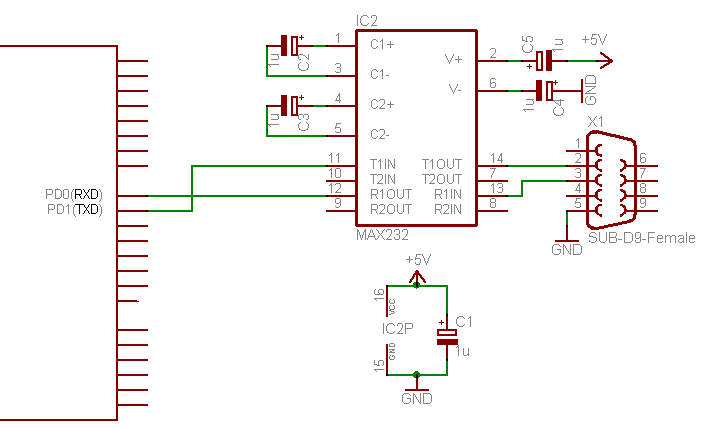
\includegraphics[width=0.6\textwidth]{AVR-RS232}
%\caption{Schema: MAX232}
%\label{fig:MAX232}
%\citep{uC:RS232}
%\end{figure}

%\section{Platinenlayout}
%Für den Mikrocontroller und seine Peripherie entwickelte ich ein Platinenlayout in der Open Source Software KiCad. \\ 
%Dazu wurden die Schaltungen wie auf dem STK500 in den Schaltplan übernommen und dort das Layout entwickelt. 
%\begin{figure}[htb]
%\centering
%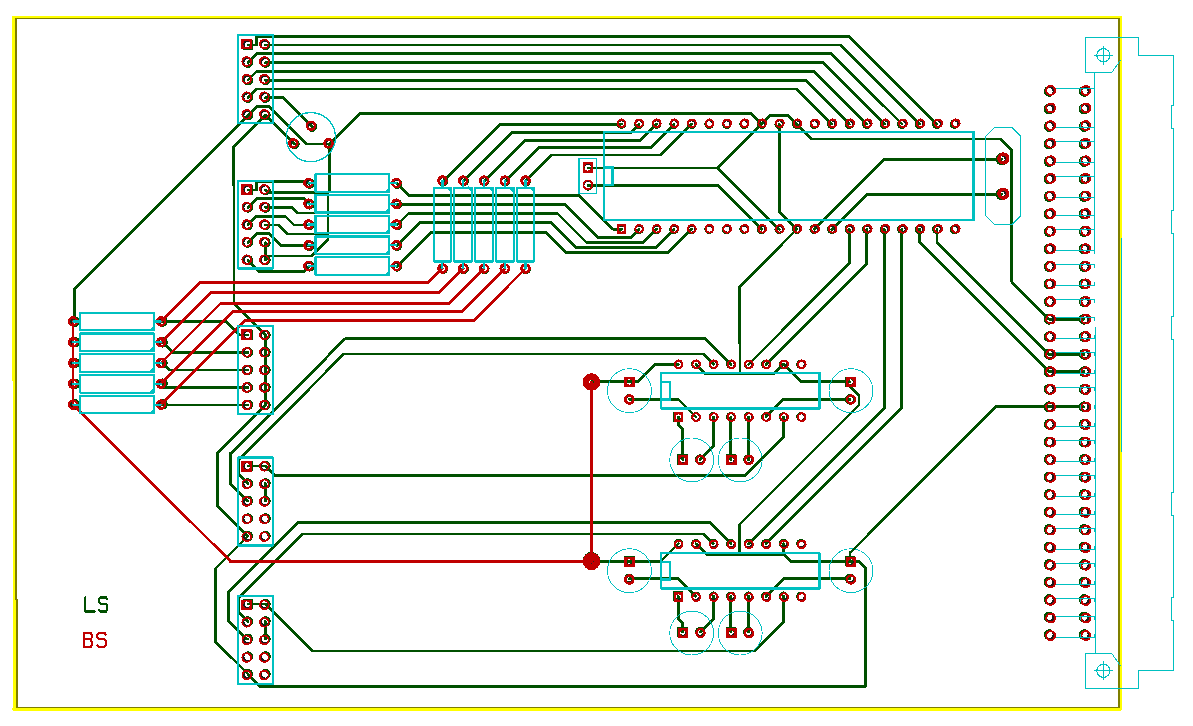
\includegraphics[width=\textwidth]{Translator_white}
%\caption{Platinenlayout}
%\label{fig:Platine}
%\end{figure}
%\todo{Schaltplan und einbinden.}
%\section{19''-Einschub}
%Die Platine für den Mikrocontroller konstruierte ich als 19''-Einschub. Über den rückwärtigen Steckverbinder verband ich die Platine mit der Spannungsversorgung. Zusätzlich kommen hier auch die Signale der Endschalter an.
%An der Vorderseite befestigte ich eine Blende. Auf der Blende befinden sich das LC-Display, fünf Taster, 5 LEDs und 2 serielle Schnittstellen. Alle Bauteile sind steckbar mit der Platine verbunden. \todo{Bild des Einschub}